%!TEX program = lualatex

\documentclass[a4paper,12pt,oneside]{book}
\usepackage[utf8]{inputenc}
\usepackage{graphicx}
\usepackage{markdown}
\usepackage{fancybox}
\usepackage{titlesec}
\usepackage{tikz}
\usepackage{geometry}
\usepackage[english]{babel}
\usepackage{blindtext}
\usepackage[titles]{tocloft}
\usepackage{xurl}
\usepackage[hidelinks]{hyperref}
\usepackage{tabularx}
\usepackage{pdfpages}
\usepackage{multicol}

\geometry{
	a4paper,
	inner=0.75in,
	top=0.75in,
	bottom=0.75in,
	outer=0.75in
}

% === TITLE FORMATTING ===
\titleformat{\chapter}[block]
{\bfseries\Large}
{\raisebox{-0.75em}{\shadowbox{\Huge \thechapter}}}
{0.5em}
{\hfill\huge}

\titlespacing{\chapter}{0em}{0em}{2em}
\titlespacing{\section}{0em}{0em}{0.5em}

% === TEXT FORMATTING ===
\setlength{\fboxsep}{1em}

\newcommand{\nurl}[1]{
  \href{#1}{\url{#1}}
}

\setlength\itemsep{0.2em}

% === STAR RATING ===
\usetikzlibrary{shapes.geometric}
\newcommand{\Stars}[2][fill=black,draw=black]
{
	\begin{tikzpicture}[baseline=-0.35em,#1]
	\foreach \X in {1,...,5}
	{
		\pgfmathsetmacro{\xfill}{min(1,max(1+#2-\X,0))}
		\path (\X*1.1em,0) 
		node[star,draw,star point height=0.25em,minimum size=1em,inner sep=0pt,
		path picture={\fill (path picture bounding box.south west) 
		rectangle  ([xshift=\xfill*1em]path picture bounding box.north west);}]{};
	}
	\end{tikzpicture}
}

% === PUZZLE MACROS ===
\newcommand{\puzzleinfo}[2]
{
	\noindent
	\emph{#1} \hfill \Stars{#2}
	\vspace{0.2em}
	\hrule
	\vspace{0.5em}
}

\newcommand{\puzzleimage}[2][0.7]
{\begin{center}
	\includegraphics[width=#1\textwidth]{#2}
\end{center}}

\newenvironment{puzzlelinks}
{
  \begin{tabularx}{\textwidth}{l X}
}
{
  \end{tabularx}
}

% === DOCUMENT ===
\begin{document}

\author{CTC Community}
\title{10,000 Archive Puzzles Pack}
\date{June 2023}

\frontmatter
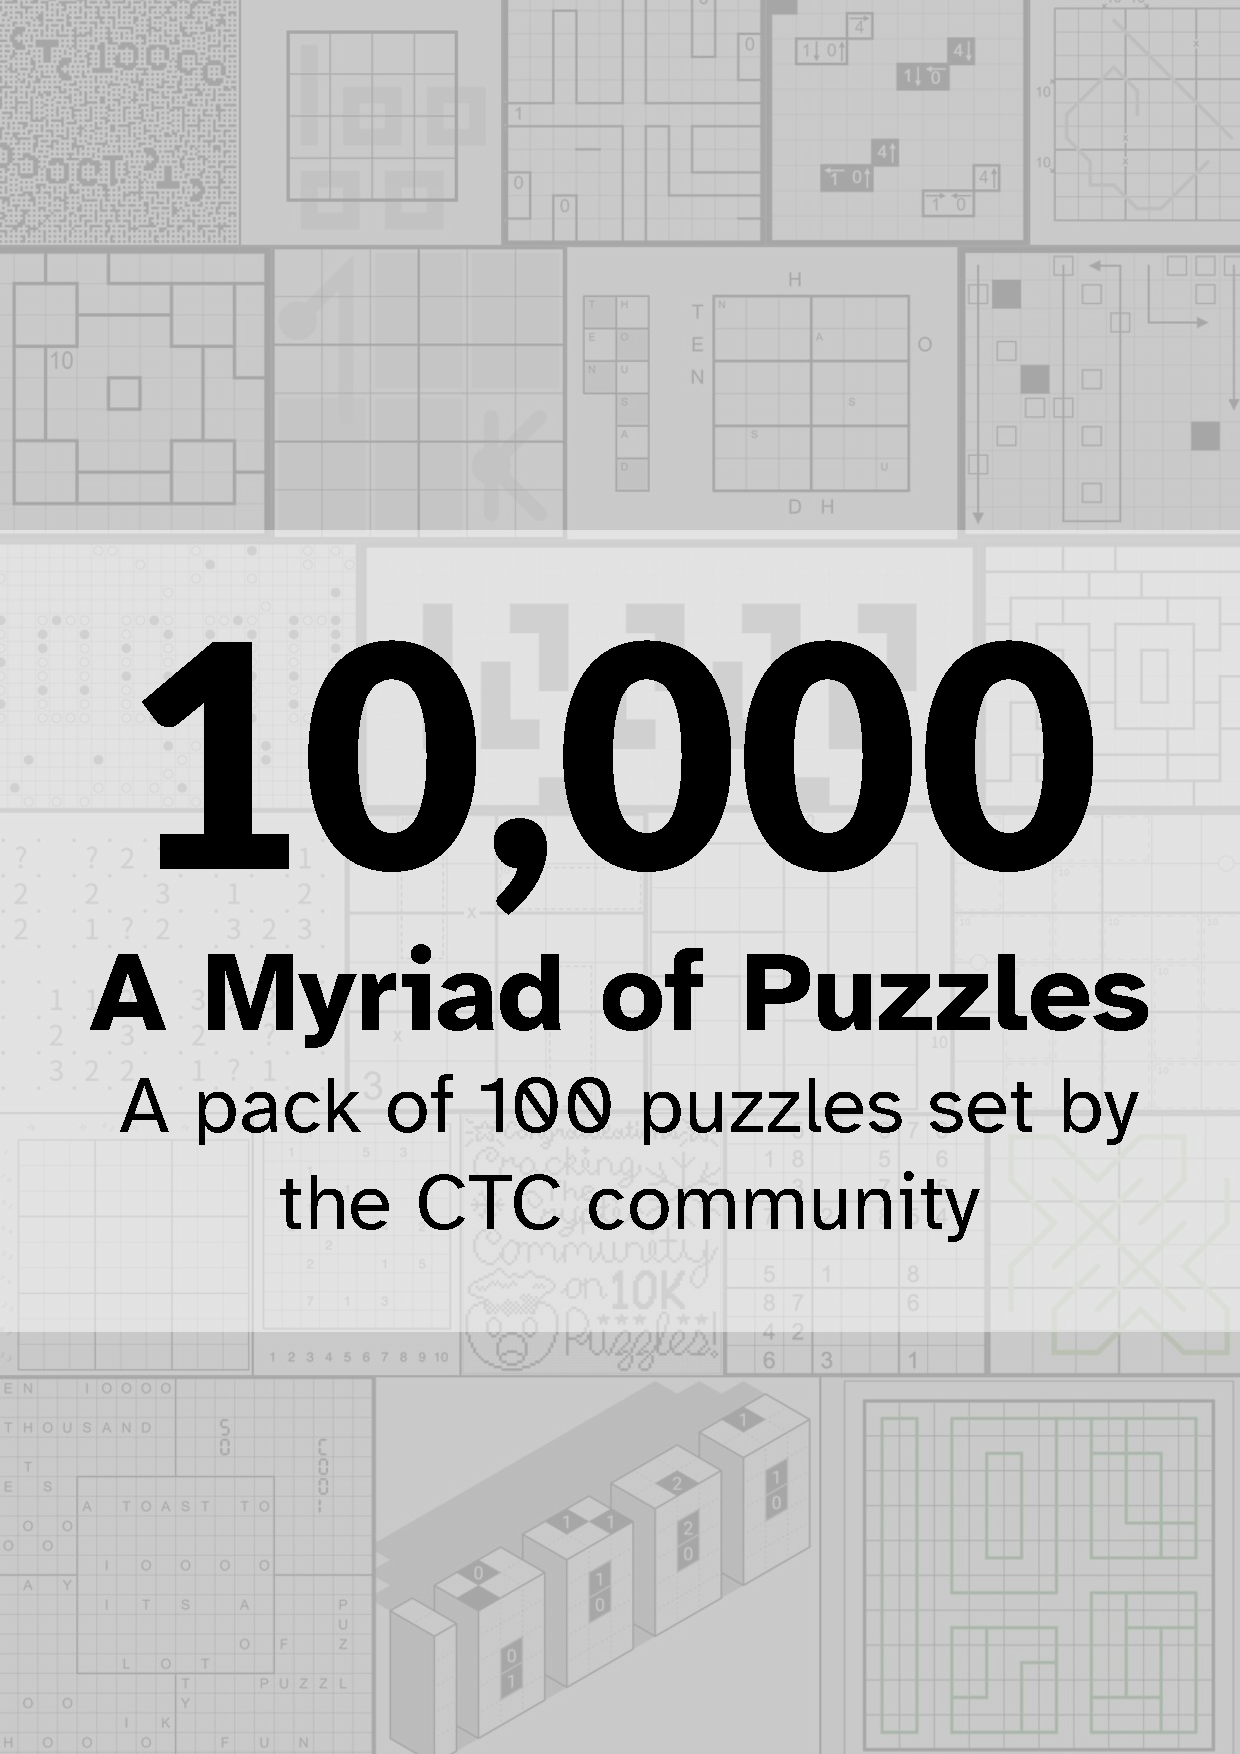
\includepdf[pages=-]{cover.pdf}
\chapter{Introduction}

In just above 3 years, this community has submitted 10,000 puzzles\footnote{Actually, it's a bit 
more than that --- there were some puzzle packs in the archive, but this pack is the 10,000th entry 
to the archive.} to the CTC Discord Archive! That's a mind boggling number of puzzles. 

To celebrate, a whole bunch of setters have come together to create a pack of $\sqrt{10000} =$ \textbf{100 puzzles}! 
They come in all kinds of genres, sizes, and difficulties, so there should be something for everyone.
When we first started this project, we didn't know yet whether we'd be able to pull it off. But in
the end, it went relatively smoothly. But was it a \emph{good} pack? We'll let you be the judge.

% This document has divided the puzzles into several categories: 
% \begin{enumerate}
%   \item \emph{Sudoku and Latin Square.} 
%   \item \emph{Loop and Path.} Basically, puzzles where your goal is to draw a line! This includes 
%       genres like Masyu, Simple Loop, or Slitherlink.
%   \item \emph{Object Placement.} 
%   \item \emph{Region Division.} 
%   \item \emph{Shading.} 
%   \item \emph{Others.}
% \end{enumerate}
% Sudoku is, of course, the thing that the CTC YouTube channel and this server is most known for. 
% It's also the largest chapter in the pack by puzzle count, which is why I decided to make it the 
% first chapter.

All of the puzzles in this pack are independent of each other, unless explicitly mentioned (in DiMono's
four puzzles, specifically), so you may solve as few/many as you want, and in any order. Here are some ideas:
\begin{itemize}
  \item Do a 100\% completion of the pack.
  \item Print it out and forget about it.
  \item Solve exactly 1 puzzle in the whole pack.
  \item Decide that you don't like Sudoku, and solve everything except for Chapter 1.
  \item Roll a d100 and solve the puzzle that corresponds to the number rolled, then repeat until satisfied.
\end{itemize}

Thank you to everyone in the server who has made this community as awesome as it is, and thank you to Mark 
and Simon for bringing us together. Here's to another 10,000 great puzzles!

\vspace{2em}

\hfill \emph{- Lavaloid}

\tableofcontents

\mainmatter
\setlength{\parindent}{0em}
\chapter{Sudoku and Latin Square}
\section{10 kage | {\normalfont Malrog}}
\label{sec:53-10-kage-malrog}
\puzzleinfo{6\emph{x}6 Sudoku, Whispers, Killer Cage}{2.0}

\puzzleimage{./puzzle_images/53-10-kage-malrog}
\subsection*{Rules}
\begin{markdown}
Standard 6x6 sudoku rules apply.

Adjacent digits on a green line must differ by at least 3.

Digits in the cage must sum to the total given.
\end{markdown}
\subsection*{Links}
\begin{tabularx}{\textwidth}{l X}
\emph{SudokuPad} & \url{https://tinyurl.com/3p329y7h} \\
\emph{F-puzzles} & \url{https://f-puzzles.com/?id=2nu8nqpr} \\
\end{tabularx}
\pagebreak

\section{10,000 Hedge Maze | {\normalfont TopAutism}}
\label{sec:52-10000-hedge-maze-topautism}
\puzzleinfo{Factorization Puzzle}{2.0}

\puzzleimage{./puzzle_images/52-10000-hedge-maze-topautism}
\subsection*{Rules}
\begin{markdown}
Place 1-6 once each in every row, column, and box.

For each line:

- For each box the line passes through:

- - Sum the digits on that line on that box.

- Multiply those sums together.

- The result must equal 10,000.
\end{markdown}
\subsection*{Links}
\begin{tabularx}{\textwidth}{l X}
\emph{CTC App} & \url{https://tinyurl.com/2s4jurm2} \\
\emph{F-puzzles} & \url{https://f-puzzles.com/?id=2zzu7lme} \\
\end{tabularx}
\pagebreak

\section[10000 Parity Little Killer | Aspartagcus {[\emph{Parity Little Killer Sudoku}]}]{10000 Parity Little Killer | {\normalfont Aspartagcus}}
\label{sec:47-10000-parity-little-killer-aspartagcus}
\puzzleinfo{Parity Little Killer Sudoku}{1.5}

\puzzleimage{./puzzle_images/47-10000-parity-little-killer-aspartagcus}
\subsection*{Rules}
\begin{markdown}
- Standard sudoku rules apply.

- Clues outside the grid give the sum of either the odd or the even digits in the indicated diagonal.

- One of the clues indicates the sum of the odd digits in its indicated diagonal, **as well as** the sum of the even digits in the diagonal.
\end{markdown}
\subsection*{Links}
\begin{tabularx}{\textwidth}{l X}
\emph{SudokuPad} & \url{https://tinyurl.com/3eaxt29a} \\
\end{tabularx}
\pagebreak

\section[10000 Product Killer | Aspartagcus {[\emph{Product Killer Sudoku}]}]{10000 Product Killer | {\normalfont Aspartagcus}}
\label{sec:53-10000-product-killer-aspartagcus}
\puzzleinfo{Product Killer Sudoku}{2.0}

\puzzleimage{./puzzle_images/53-10000-product-killer-aspartagcus}
\subsection*{Rules}
\begin{markdown}
- Standard sudoku rules apply.

- Digits in a cage either sum or multiply to the number in the corner of the cage. Digits may repeat in a cage.
\end{markdown}
\subsection*{Links}
\begin{tabularx}{\textwidth}{l X}
\emph{SudokuPad} & \url{https://tinyurl.com/mta6k8c3} \\
\end{tabularx}
\pagebreak

\section[10000 killers in the fog | Aspartagcus {[\emph{Irregular Killer Fog Of War Sudoku}]}]{10000 killers in the fog | {\normalfont Aspartagcus}}
\label{sec:43-10000-killers-in-the-fog-aspartagcus}
\puzzleinfo{Irregular Killer Fog Of War Sudoku}{3.5}

\puzzleimage{./puzzle_images/43-10000-killers-in-the-fog-aspartagcus}
\subsection*{Rules}
\begin{markdown}
- 8x8 irregular sudoku rules apply.

- Digits in a cage do not repeat and sum to 10.

- Most of the clues are hidden in fog, enter correct digits to disperse it.
\end{markdown}
\subsection*{Links}
\begin{tabularx}{\textwidth}{l X}
\emph{SudokuPad} & \url{https://tinyurl.com/5n7ck94k} \\
\end{tabularx}
\pagebreak

\section{10000 with a k | {\normalfont Ymmi}}
\label{sec:05-10000-with-a-k-ymmi}
\puzzleinfo{Sudoku}{1.5}

\puzzleimage{./puzzle_images/05-10000-with-a-k-ymmi}
\subsection*{Rules}
\begin{markdown}
Normal sudoku rules apply.

Antiknight: Two cells spanned by a knight's move must not contain the same digit.

Extra region: Each grey region contains one set of the digits 1 to 6.

Thermos: Digits along the thermometer must increase from the bulb end.
\end{markdown}
\subsection*{Links}
\begin{tabularx}{\textwidth}{l X}
\emph{F-puzzles} & \url{https://f-puzzles.com/?id=27hm95mx} \\
\end{tabularx}
\pagebreak

\section[10Khaos | MicroStudy {[\emph{Sudoku, Chaos Construction, X-Sums}]}]{10Khaos | {\normalfont MicroStudy}}
\label{sec:28-10khaos-microstudy}
\puzzleinfo{Sudoku, Chaos Construction, X-Sums}{1.5}

\puzzleimage{./puzzle_images/28-10khaos-microstudy}
\subsection*{Rules}
\begin{markdown}
Chaos Construction (6x6): Divide the grid into regions, each consisting of six orthogonally connected cells. Each row, column and region must contain the digits 1-6 once each.



X-Sums: Clues outside the grid show the sum of the first X cells in the corresponding row/column, where X is the digit in the cell nearest to the clue. In addition, the first X cells in this row/column are part of the same region, and the X+1th cell is part of a different region. ? clues can stand for any positive integer.
\end{markdown}
\subsection*{Links}
\begin{tabularx}{\textwidth}{l X}
\emph{SudokuPad} & \url{https://tinypuz.com/2k79cwh9} \\
\end{tabularx}
\pagebreak

\section{10Konstraints | {\normalfont SSG}}
\label{sec:35-10konstraints-ssg}
\puzzleinfo{Multi-Variant Sudoku}{3.5}

\puzzleimage{./puzzle_images/35-10konstraints-ssg}
\subsection*{Rules}
\begin{markdown}
Normal sudoku rules apply.



**Arrow**: Digits along an arrow must sum to the digit in the connected circle.



**Consecutive Pairs**: Cells connected by a white dot must contain consecutive digits.



**Entropic Lines**: Along a beige line any run of three cells must contain one low {1,2,3}, one medium {4,5,6}, and one high {7,8,9} digit.



**German Whispers**: Successive digits along a green line must differ by at least 5.



**Ratio Pairs**: Cells connected by a black dot must contain digits in a ratio of 1:2.



**Renban**: Each purple line must contain a non-repeating set of consecutive digits which may appear in any order.



**Sandwich**: Uncircled clues outside the grid give the sum of the digits placed between the 1 and 9 in that row or column.



**Thermo**: Digits along a thermometer must strictly increase starting at the bulb.



**X Pairs**: Cells connected by an X must contain digits summing to 10.



**X-Sums**: Circled clues outside the grid give the sum of the first X digits from the position of the clue, where X is the first digit encountered.
\end{markdown}
\subsection*{Links}
\begin{tabularx}{\textwidth}{l X}
\emph{F-puzzles} & \url{https://f-puzzles.com/?id=2gaqeurn} \\
\emph{CTC App} & \url{https://tinyurl.com/2ae6v74y} \\
\end{tabularx}
\pagebreak

\section{10k (Not) In a Row | {\normalfont SSG}}
\label{sec:35-10k-not-in-a-row-ssg}
\puzzleinfo{Non-Consecutive Sudoku}{1.0}

\puzzleimage{./puzzle_images/35-10k-not-in-a-row-ssg}
\subsection*{Rules}
\begin{markdown}
Place the digits 0-5 once each in each row, column, and 2x3 box.



**Non-Consecutive**: Orthogonally adjacent cells may not contain consecutive digits.
\end{markdown}
\subsection*{Links}
\begin{tabularx}{\textwidth}{l X}
\emph{Penpa+} & \url{https://tinyurl.com/4393b7ey} \\
\emph{CTC App} & \url{https://tinyurl.com/yc2x4vxv} \\
\end{tabularx}
\pagebreak

\section{10k Equalines | {\normalfont Xendari}}
\label{sec:39-10k-equalines-xendari}
\puzzleinfo{Sudoku, Equalines}{2.0}

\puzzleimage{./puzzle_images/39-10k-equalines-xendari}
\subsection*{Rules}
\begin{markdown}
Normal sudoku rules apply.



Digits on each line must sum to the same number. Digits may repeat on a line where allowed by other rules.
\end{markdown}
\subsection*{Links}
\begin{tabularx}{\textwidth}{l X}
\emph{SudokuPad} & \url{https://tinyurl.com/5d8m6z4w} \\
\end{tabularx}
\pagebreak

\section[10k Irregular Killer | Aspartagcus {[\emph{Irregular Killer Sudoku}]}]{10k Irregular Killer | {\normalfont Aspartagcus}}
\label{sec:44-10k-irregular-killer-aspartagcus}
\puzzleinfo{Irregular Killer Sudoku}{1.5}

\puzzleimage{./puzzle_images/44-10k-irregular-killer-aspartagcus}
\subsection*{Rules}
\begin{markdown}
- Irregular 6x6 sudoku rules apply. A couple of regions have been separated into smaller, unconnected areas, but each region is still made up of 6 cells.

- Digits in a cage do not repeat and sum to 10.
\end{markdown}
\subsection*{Links}
\begin{tabularx}{\textwidth}{l X}
\emph{SudokuPad} & \url{https://tinyurl.com/y7m7c5df} \\
\end{tabularx}
\pagebreak

\section{20000 Truths and 10000 Lies | {\normalfont MicroStudy}}
\label{sec:41-20000-truths-and-10000-lies-microstudy}
\puzzleinfo{Sudoku, Liar Clues, German Whispers, Renban, Kropki Pairs}{3.5}

\puzzleimage{./puzzle_images/41-20000-truths-and-10000-lies-microstudy}
\subsection*{Rules}
\begin{markdown}
Normal 6x6 Sudoku rules apply: Place the digits 1-6 once each into every row, column and 2x3 box.



Standard variant rules apply. However, exactly one instance of each given clue type is incorrect. There are no negative constraints.



Standard variant clue types included: Black Kropki Dots, White Kropki Dots, German Whispers (difference of >=3), Renban



Detailed Variant Rules:

- Black Kropki Dots: Digits separated by a black Kropki dot must be in a ratio of 1:2.

- White Kropki Dots: Digits separated by a white Kropki dot must be consecutive.

- German Whispers (6x6): Adjacent digits along a green German Whispers line must differ by 3 or more.

- Renban: Digits along a purple Renban line must form a set of consecutive, non-repeating digits in any order.
\end{markdown}
\subsection*{Links}
\begin{tabularx}{\textwidth}{l X}
\emph{CTC App} & \url{https://tinyurl.com/45nvwt5c} \\
\end{tabularx}
\pagebreak

\section{A 10 Dance | {\normalfont SSG}}
\label{sec:35-a-10-dance-ssg}
\puzzleinfo{Killer/Little Killer Sudoku}{3.5}

\puzzleimage[0.8]{./puzzle_images/35-a-10-dance-ssg}
\subsection*{Rules}
\begin{markdown}
Normal sudoku rules apply.



**Killer**: Digits may not repeat in cages and must sum to the given total.



**Little Killer**: Digits along an indicated diagonal must sum to the given total and may repeat if allowed by other rules.
\end{markdown}
\subsection*{Links}
\begin{tabularx}{\textwidth}{l X}
\emph{F-puzzles} & \url{https://f-puzzles.com/?id=2mldl92a} \\
\emph{CTC App} & \url{https://tinyurl.com/47hz3c4f} \\
\end{tabularx}
\pagebreak

\section[Ambiguous 10k thermometers | Aspartagcus {[\emph{Thermo Sudoku}]}]{Ambiguous 10k thermometers | {\normalfont Aspartagcus}}
\label{sec:11-ambiguous-10k-thermometers-aspartagcus}
\puzzleinfo{Thermo Sudoku}{1.5}

\puzzleimage{./puzzle_images/11-ambiguous-10k-thermometers-aspartagcus}
\subsection*{Rules}
\begin{markdown}
- Standard 6x6 sudoku rules apply.

- Digits increase from the bulb to the tip of each thermometer. The location of the tips of the thermometers need to be disambiguated by the solver.
\end{markdown}
\subsection*{Links}
\begin{tabularx}{\textwidth}{l X}
\emph{SudokuPad} & \url{https://tinyurl.com/5n875un9} \\
\end{tabularx}
\pagebreak

\section[Blackbird Pie | jubale, Malrog {[\emph{10\emph{x}10 Latin Square, Deficit, Killer Cages}]}]{Blackbird Pie | {\normalfont jubale, Malrog}}
\label{sec:09-blackbird-pie-jubale-malrog}
\puzzleinfo{10\emph{x}10 Latin Square, Deficit, Killer Cages}{4.0}
Sing a song of six pence, a 10x10 Sudoku.

Four tens, twenty cages baked just for you!

Hope you solve the tricky bits, or at least you give a try.

But work this puzzle carefully, it’s easy to go awry.
\puzzleimage[0.9]{./puzzle_images/09-blackbird-pie-jubale-malrog}
\subsection*{Rules}
\begin{markdown}
Place 1-10 once each in every row and column.  Numbers may not repeat within a 3x3 box.  Numbers in cages may not repeat and sum to the value in the corner.

Solving note: Use 0 in place of 10 if solving in SudokuPad, its value still counts as 10 for cages.
\end{markdown}
\subsection*{Links}
\begin{tabularx}{\textwidth}{l X}
\emph{F-puzzles} & \url{https://f-puzzles.com/?id=2fwdh9yj} \\
\emph{SudokuPad} & \url{https://tinyurl.com/424bcbtc} \\
\end{tabularx}
\pagebreak

\section[Congrats on 10k | Panthera {[\emph{JSS/Sandwich}]}]{Congrats on 10k | {\normalfont Panthera}}
\label{sec:52-congrats-on-10k-panthera}
\puzzleinfo{JSS/Sandwich}{1.0}

\puzzleimage[0.85]{./puzzle_images/52-congrats-on-10k-panthera}
\subsection*{Rules}
\begin{markdown}
Normal sudoku rules apply.

Adjusted Japanese sums rules apply.



Normal Japanese Sums: The clues outside the grid indicate the sums of the contiguous runs found in that row or column that must be shaded. There must be an unshaded cell between runs of the same color. If a row or column is unclued, there is no shading in that row or column.



Adjusted -- any outside clue could represent a sandwich clue instead! (that is, the sum of the digits between the 1 and 9 where the 1, 9, and all the digits in between are shaded). 
\end{markdown}
\subsection*{Links}
\begin{tabularx}{\textwidth}{l X}
\emph{CTC} & \url{https://tinyurl.com/4p5rnb7w} \\
\end{tabularx}
\pagebreak

\section{DecaDots | {\normalfont SSG}}
\label{sec:31-decadots-ssg}
\puzzleinfo{Kropki Pairs Sudoku}{1.0}

\puzzleimage{./puzzle_images/31-decadots-ssg}
\subsection*{Rules}
\begin{markdown}
Normal 6x6 sudoku rules apply.



**Kropki Pairs**: Cells connected by a white dot must contain consecutive digits. Cells connected by black dots must contain digits in a 1:2 ratio. Not all possible dots are necessarily given.
\end{markdown}
\subsection*{Links}
\begin{tabularx}{\textwidth}{l X}
\emph{F-puzzles} & \url{https://f-puzzles.com/?id=2oytpytl} \\
\emph{CTC App} & \url{https://tinyurl.com/2efn5c8f} \\
\end{tabularx}
\pagebreak

\section[Four Diamonds | TopAutism {[\emph{Parity}]}]{Four Diamonds | {\normalfont TopAutism}}
\label{sec:10-four-diamonds-topautism}
\puzzleinfo{Parity}{2.0}
Parity coloring puzzle based on diamond shapes.

\puzzleimage{./puzzle_images/10-four-diamonds-topautism}
\subsection*{Rules}
\begin{markdown}
Place 1-6 once each in every row, column, and box.

Digits in a cage sum to the clue in the top left corner.

Digits on yellow lines alternate odd & even.

On the red line, consecutive digits are consecutive.
\end{markdown}
\subsection*{Links}
\begin{tabularx}{\textwidth}{l X}
\emph{SudokuPad} & \url{https://tinyurl.com/mr2xdxnx} \\
\emph{F-puzzles} & \url{https://f-puzzles.com/?id=2droq655} \\
\end{tabularx}
\pagebreak

\section[Irregular reg10n sums | Aspartagcus {[\emph{5\emph{x}5 Irregular Region Sums Sudoku}]}]{Irregular reg10n sums | {\normalfont Aspartagcus}}
\label{sec:37-irregular-reg10n-sums-aspartagcus}
\puzzleinfo{5\emph{x}5 Irregular Region Sums Sudoku}{1.0}

\puzzleimage{./puzzle_images/37-irregular-reg10n-sums-aspartagcus}
\subsection*{Rules}
\begin{markdown}
- Place the digits 1-5 once each into every row and column. Digits within regions may not repeat.

- For each line, digits on the line have an equal sum N within each box it passes through. Different lines may have different sums.
\end{markdown}
\subsection*{Links}
\begin{tabularx}{\textwidth}{l X}
\emph{SudokuPad} & \url{https://tinyurl.com/mmuzhypn} \\
\end{tabularx}
\pagebreak

\section{Killing it at 10k | {\normalfont Degustaf}}
\label{sec:34-killing-it-at-10k-degustaf}
\puzzleinfo{Killer Mean Mini Sudoku}{2.0}

\puzzleimage{./puzzle_images/34-killing-it-at-10k-degustaf}
\subsection*{Rules}
\begin{markdown}
Place 6 of the digits from 1 to 9 into the grid so that no digit repeats in any row, column, or box.

Digits in a cage must sum to the total given in the corner.

Digits separated by a white kropki dot must be consecutive.
\end{markdown}
\subsection*{Links}
\begin{tabularx}{\textwidth}{l X}
\emph{SudokuPad} & \url{https://tinyurl.com/4wbzeznb} \\
\end{tabularx}
\pagebreak

\section{Kr0000pki D0000ts | {\normalfont MicroStudy}}
\label{sec:24-kr0000pki-d0000ts-microstudy}
\puzzleinfo{Sudoku, Kropki Pairs, Kroopki Doots}{2.0}

\puzzleimage{./puzzle_images/24-kr0000pki-d0000ts-microstudy}
\subsection*{Rules}
\begin{markdown}
Normal 6x6 Sudoku rules apply. Place the digits 1-6 once each into every row, column and 2x3 box.



Kropki Dots: Digits separated by a white Kropki dot must be consecutive. Digits separated by a black Kropki dot must have a ratio of 1:2. Not all Kropki dots are necessarily given.



Kroopki Doots: Sets of digits separated by a white Kroopki doot (the long, ellipse-looking things) must have their respective sums be consecutive. Sets of digits separated by a black Kroopki doot must have their respective sums be in a 1:2 ratio. Not all Kroopki doots are given.
\end{markdown}
\subsection*{Links}
\begin{tabularx}{\textwidth}{l X}
\emph{CTC App} & \url{https://tinyurl.com/yp6hhhhz} \\
\end{tabularx}
\pagebreak

\section{loooo | {\normalfont Lavaloid}}
\label{sec:18-loooo-lavaloid}
\puzzleinfo{Renban Skyscrapers}{3.5}

\puzzleimage{./puzzle_images/18-loooo-lavaloid}
\subsection*{Rules}
\begin{markdown}
*Skyscraper:* Place a number from 1 to N into each cell so that each row and column contains every number from that range with no repeats, where N is the side length of the grid. A clue outside the grid represents how many cells in the corresponding row or column contain a larger number than all cells before it in that row or column from the direction of the clue.



*Renban:* Digits along the given lines must form a non-repeating consecutive group of numbers in any order. Some of the digits may be outside the grid, where they behave as skyscrapers clues.



**Solving note:** For answer check, fill in all cells with cages.
\end{markdown}
\subsection*{Links}
\begin{tabularx}{\textwidth}{l X}
\emph{Penpa+} & \url{https://tinyurl.com/2gcbjbtx} \\
\end{tabularx}
\pagebreak

\section{Mounted Archers | {\normalfont DiMono}}
\label{sec:20-mounted-archers-dimono}
\puzzleinfo{6\emph{x}6 Irregular Anti-Knight Little Killer}{1.5}
The first of four in a set
\puzzleimage{./puzzle_images/20-mounted-archers-dimono}
\subsection*{Rules}
\begin{markdown}
Irregular 6x6: Place the numbers 1-6 into each row, column, and region, exactly once.



Anti-knight: Cells separated by a knight's move must contain different digits.



Little Killer: Digits along an indicated diagonal must sum to the value of the clue.
\end{markdown}
\subsection*{Links}
\begin{tabularx}{\textwidth}{l X}
\emph{F-puzzles} & \url{https://f-puzzles.com/?id=2mxb5kzu} \\
\emph{CTC App} & \url{https://tinyurl.com/MountedArchers} \\
\end{tabularx}
\pagebreak

\section[Mobile Oubliettes | DiMono {[\emph{Irregular 6\emph{x}6 Anti-Knight Killer}]}]{Mobile Oubliettes | {\normalfont DiMono}}
\label{sec:58-mobile-oubliettes-dimono}
\puzzleinfo{Irregular 6\emph{x}6 Anti-Knight Killer}{1.5}
The second of four
\puzzleimage{./puzzle_images/58-mobile-oubliettes-dimono}
\subsection*{Rules}
\begin{markdown}
Irregular 6x6: Place the numbers 1-6 into each row, column, and region, exactly once.



Anti-knight: Cells separated by a knight's move must contain different digits.



Killer Cages: Cells inside a cage must sum to the total in the top left of the cage without repeating any digits.
\end{markdown}
\subsection*{Links}
\begin{tabularx}{\textwidth}{l X}
\emph{F-puzzles} & \url{https://f-puzzles.com/?id=2f6fnhux} \\
\emph{CTC App} & \url{https://tinyurl.com/MobileOubliettes} \\
\end{tabularx}
\pagebreak

\section[Mounted Divisions | DiMono {[\emph{6\emph{x}6 Irregular Anti-Knight Region Sum Lines}]}]{Mounted Divisions | {\normalfont DiMono}}
\label{sec:50-mounted-divisions-dimono}
\puzzleinfo{6\emph{x}6 Irregular Anti-Knight Region Sum Lines}{2.0}
The third of four
\puzzleimage{./puzzle_images/50-mounted-divisions-dimono}
\subsection*{Rules}
\begin{markdown}
Irregular 6x6: Place the numbers 1-6 into each row, column, and region, exactly once.



Anti-knight: Cells separated by a knight's move must contain different digits.



Region Sum Lines: Digits on a blue line add to the same sum in each box the line appears in.
\end{markdown}
\subsection*{Links}
\begin{tabularx}{\textwidth}{l X}
\emph{F-puzzles} & \url{https://f-puzzles.com/?id=2xzh6la2} \\
\emph{CTC App} & \url{https://tinyurl.com/MountedDivisions} \\
\end{tabularx}
\pagebreak

\section[Same As It Ever Was | DiMono {[\emph{6\emph{x}6 Irregular Anti-Knight X-Sums + Deja Vu}]}]{Same As It Ever Was | {\normalfont DiMono}}
\label{sec:09-same-as-it-ever-was-dimono}
\puzzleinfo{6\emph{x}6 Irregular Anti-Knight X-Sums + Deja Vu}{2.0}
The fourth of four.
\puzzleimage{./puzzle_images/09-same-as-it-ever-was-dimono}
\subsection*{Rules}
\begin{markdown}
Irregular 6x6: Place the numbers 1-6 into each row, column, and region, exactly once.



Anti-knight: Cells separated by a knight's move must contain different digits.



X-Sums: Clues outside the grid indicate the sum of the first X cells that are "seen" from the clue, where X is the digit in the first seen cell.



Deja Vu: This puzzle has a unique solution - if you've been paying attention to my puzzles in this pack.
\end{markdown}
\subsection*{Links}
\begin{tabularx}{\textwidth}{l X}
\emph{F-puzzles} & \url{https://f-puzzles.com/?id=23o29sua} \\
\emph{CTC App} & \url{https://tinyurl.com/CTCSameAsItEverWas} \\
\end{tabularx}
\pagebreak

\section[No Deficit of Puzzles | rockratzero {[\emph{Deficit Killer Sudoku}]}]{No Deficit of Puzzles | {\normalfont rockratzero}}
\label{sec:04-no-deficit-of-puzzles-rockratzero}
\puzzleinfo{Deficit Killer Sudoku}{2.5}

\puzzleimage{./puzzle_images/04-no-deficit-of-puzzles-rockratzero}
\subsection*{Rules}
\begin{markdown}
7x7 Latin Square Rules Apply. Place the digits 1-7 in each row and column without repeating. 

Additionally, no digit may repeat within a bold bordered region. 

Digits in cages sum to 10.
\end{markdown}
\subsection*{Links}
\begin{tabularx}{\textwidth}{l X}
\emph{SudokuPad} & \url{https://tinyurl.com/29w429z8} \\
\end{tabularx}
\pagebreak

\section[Production Lines | James Sinclair {[\emph{Sudoku}]}]{Production Lines | {\normalfont James Sinclair}}
\label{sec:25-production-lines-james-sinclair}
\puzzleinfo{Sudoku}{1.5}

\puzzleimage[0.9]{./puzzle_images/25-production-lines-james-sinclair}
\subsection*{Rules}
\begin{markdown}
Normal sudoku rules apply. The product of the digits along each gray line is 10,000. Clues outside the grid give the sum of the digits along the indicated diagonal. Digits in cells separated by an X sum to 10.
\end{markdown}
\subsection*{Links}
\begin{tabularx}{\textwidth}{l X}
\emph{F-puzzles} & \url{https://f-puzzles.com/?id=2nuxkjug} \\
\emph{SudokuPad} & \url{https://tinyurl.com/3fdr4pe2} \\
\end{tabularx}
\pagebreak

\section[Small Differences | jubale {[\emph{Sudoku, Subtraction Arrows}]}]{Small Differences | {\normalfont jubale}}
\label{sec:31-small-differences-jubale}
\puzzleinfo{Sudoku, Subtraction Arrows}{2.0}

\puzzleimage{./puzzle_images/31-small-differences-jubale}
\subsection*{Rules}
\begin{markdown}
Place 0-5 in each row, column, and box without repeats.

Arrows are subtraction defined by BULB = MIDDLE - TIP.
\end{markdown}
\subsection*{Links}
\begin{tabularx}{\textwidth}{l X}
\emph{SudokuPad} & \url{https://tinypuz.com/2xht3ete} \\
\emph{Penpa+} & \url{https://tinyurl.com/2c5qqre4} \\
\end{tabularx}
\pagebreak

\section{Su10ku! | {\normalfont SSG}}
\label{sec:28-su10ku-ssg}
\puzzleinfo{Classic Sudoku}{1.0}

\puzzleimage{./puzzle_images/28-su10ku-ssg}
\subsection*{Rules}
\begin{markdown}
Normal sudoku rules apply.
\end{markdown}
\subsection*{Links}
\begin{tabularx}{\textwidth}{l X}
\emph{CTC App} & \url{https://tinyurl.com/6n76punx} \\
\emph{F-puzzles} & \url{https://f-puzzles.com/?id=2d4aupae} \\
\end{tabularx}
\pagebreak

\section{TEN HOUSAD | {\normalfont Xendari}}
\label{sec:08-ten-housad-xendari}
\puzzleinfo{Sudoku, X-Sums, Cipher}{2.0}

\puzzleimage[1]{./puzzle_images/08-ten-housad-xendari}
\subsection*{Rules}
\begin{markdown}
Normal 6x6 sudoku rules apply.

Each letter represents a different number from 1-9. Clues outside the grid give the sum of the first X cells in that direction, where X is the first cell seen from that direction. A cell with a letter must contain its associated digit.
\end{markdown}
\subsection*{Links}
\begin{tabularx}{\textwidth}{l X}
\emph{Penpa+} & \url{https://tinyurl.com/dm39rn8e} \\
\end{tabularx}
\pagebreak

\section[Ten(sions in the dar)K | MicroStudy {[\emph{Sudoku, Fog Of War, Killer, Kropki Pairs}]}]{Ten(sions in the dar)K | {\normalfont MicroStudy}}
\label{sec:08-ten-sions-in-the-dar-k-microstudy}
\puzzleinfo{Sudoku, Fog Of War, Killer, Kropki Pairs}{2.0}

\puzzleimage{./puzzle_images/08-ten-sions-in-the-dar-k-microstudy}
\subsection*{Rules}
\begin{markdown}
Normal Sudoku rules apply: Place the digits 1-9 once each into every row, column and 3x3 box.



Fog of War: The grid is mostly covered in darkness. Placing correct digits illuminates adjacent cells. No guessing is required.



Killer Cages: Digits inside Killer Cages cannot repeat and must sum to the digit in the top left corner.



Kropki Pairs: Digits separated by a black dot must be in a 1:2 ratio. Digits separated by a white dot must be consecutive. Not all dots are necessarily given.
\end{markdown}
\subsection*{Links}
\begin{tabularx}{\textwidth}{l X}
\emph{CTC App} & \url{https://tinyurl.com/3u39cpu6} \\
\end{tabularx}
\pagebreak

\section{Tenban | {\normalfont jubale}}
\label{sec:44-tenban-jubale}
\puzzleinfo{Sudoku/Renban,Killer}{3.5}

\puzzleimage{./puzzle_images/44-tenban-jubale}
\subsection*{Rules}
\begin{markdown}
Place the numbers 0-5 in every row, column and 2x3 box.



Digits in a cage may not repeat, and sum to the number in the corner.



Digits on a purple renban line are consecutive, in any order.
\end{markdown}
\subsection*{Links}
\begin{tabularx}{\textwidth}{l X}
\emph{CTC App} & \url{https://tinyurl.com/2uu9nc4f} \\
\end{tabularx}
\pagebreak

\section[X-Knight | myShoggoth {[\emph{Sudoku, Killer, XV}]}]{X-Knight | {\normalfont myShoggoth}}
\label{sec:01-x-knight-myshoggoth}
\puzzleinfo{Sudoku, Killer, XV}{1.0}

\puzzleimage{./puzzle_images/01-x-knight-myshoggoth}
\subsection*{Rules}
\begin{markdown}
Normal 6x6 sudoku rules apply. The same digit may not repeat a chess knight's move apart. Digits separated by Xs must sum to 10. Digits in killer cages sum to the number in its upper left, and may not repeat. Not all Xs are necessarily given.
\end{markdown}
\subsection*{Links}
\begin{tabularx}{\textwidth}{l X}
\emph{CTC App} & \url{https://tinyurl.com/4av6bhjs} \\
\end{tabularx}
\pagebreak


\chapter{Loop and Path}
\section[10$^4$ | Malrog {[\emph{Ichimaga}]}]{10$^4$ | {\normalfont Malrog}}
\label{sec:11-10-4-malrog}
\puzzleinfo{Ichimaga}{1.5}

\puzzleimage{./puzzle_images/11-10-4-malrog}
\subsection*{Rules}
\begin{markdown}
Draw paths along the grid lines connecting pairs of circles such that all circles form one connected network. Paths may not cross each other or themselves, and a path may not turn more than once. A number in a circle indicates how many paths are connected to it.
\end{markdown}
\subsection*{Links}
\begin{tabularx}{\textwidth}{l X}
\emph{Puzz.link} & \url{https://puzz.link/p?ichimaga/10/9/tbqdbhek1.rbdqdr} \\
\end{tabularx}
\pagebreak

\section[10$^4$ Castle Wall | Stef {[\emph{Castle Wall}]}]{10$^4$ Castle Wall | {\normalfont Stef}}
\label{sec:37-104-castle-wall-stef}
\puzzleinfo{Castle Wall}{2.0}

\puzzleimage{./puzzle_images/37-104-castle-wall-stef}
\subsection*{Rules}
\begin{markdown}
Draw a single closed loop (without intersections or crossings) passing through some empty cells in the grid. The grid contains some bordered or colored cells that cannot be part of the loop. Black cells must be outside the loop; white cells (with heavy borders) must be inside the loop. Numbers and arrows refer to the total sum of the lengths of loop segments in the given direction. (An equivalent way to understand these values is to count the number of cell borders crossed by the loop in that direction.)
\end{markdown}
\subsection*{Links}
\begin{tabularx}{\textwidth}{l X}
\emph{Puzz.link} & \url{https://puzz.link/p?castle/10/10/20.l144g121110d224g221230za214g231210d114g141130l} \\
\end{tabularx}
\pagebreak

\section{10,000 Double Back | {\normalfont Danlson}}
\label{sec:20-10000-double-back-danlson}
\puzzleinfo{Double Back}{2.5}

\puzzleimage[0.9]{./puzzle_images/20-10000-double-back-danlson}
\subsection*{Rules}
\begin{markdown}
Draw a loop that goes through every unshaded cell.

1. The loop cannot branch off or cross itself.

2. The loop cannot go through shaded cells.

3. The loop visits each outlined region exactly twice.
\end{markdown}
\subsection*{Links}
\begin{tabularx}{\textwidth}{l X}
\emph{Puzz.link} & \url{https://puzz.link/p?doubleback/17/7/9h911afddnlmrrrdrq54ad07fcnsrc0h4g601sdmmvl0000000000000000000000002} \\
\end{tabularx}
\pagebreak

\section{10,000 Midloop | {\normalfont Danlson}}
\label{sec:37-10000-midloop-danlson}
\puzzleinfo{Midloop}{1.0}

\puzzleimage[1]{./puzzle_images/37-10000-midloop-danlson}
\subsection*{Rules}
\begin{markdown}
Draw lines through orthogonally adjacent cells to form a loop that goes through every circle.

1. The loop cannot branch off or cross itself.

2. Each circle marks the center of the straight line segment it lies on.
\end{markdown}
\subsection*{Links}
\begin{tabularx}{\textwidth}{l X}
\emph{Puzz.link} & \url{https://puzz.link/p?midloop/21/6/zfzzt59fiff9fzi3bfxffrbfzpfhffzz559739ff9fzzfsfl} \\
\end{tabularx}
\pagebreak

\section[10,000 Remembered Length | Danlson {[\emph{Remembered Length}]}]{10,000 Remembered Length | {\normalfont Danlson}}
\label{sec:07-10000-remembered-length-danlson}
\puzzleinfo{Remembered Length}{1.5}

\puzzleimage[1]{./puzzle_images/07-10000-remembered-length-danlson}
\subsection*{Rules}
\begin{markdown}
Draw lines through orthogonally adjacent cells to form a directional loop.

1. All unshaded cells must be visited.

2. The loop cannot branch off or cross itself.

3. Each time the loop exits a region containing a number, its visit to the next region must consist of exactly that number of cells.
\end{markdown}
\subsection*{Links}
\begin{tabularx}{\textwidth}{l X}
\emph{Puzz.link} & \url{https://puzz.link/p?remlen/17/4/i24eirf9dk888r3vh54gm6r000000000g0040012345q} \\
\end{tabularx}
\pagebreak

\section{10000 Nanameguri | {\normalfont Aspartagcus}}
\label{sec:35-10000-nanameguri-aspartagcus}
\puzzleinfo{Nanameguri}{3.5}

\puzzleimage[1]{./puzzle_images/35-10000-nanameguri-aspartagcus}
\subsection*{Rules}
\begin{markdown}
Draw a non-intersecting loop through the centers of some cells which passes through each region exactly once. Each cell containing a diagonal portion of a region boundary must be used by the loop in exactly one of the two regions it separates, and the loop must make a 90° turn, as though reflected off of it.
\end{markdown}
\subsection*{Links}
\begin{tabularx}{\textwidth}{l X}
\emph{Puzz.link} & \url{https://puzz.link/p?nanameguri/20/5/21ikc010pj6bg2412paihfk0401808huha40000000fj6b3j200000003m6b3i0000000} \\
\end{tabularx}
\pagebreak

\section[10K Road Trip | jubale {[\emph{Road Trip}]}]{10K Road Trip | {\normalfont jubale}}
\label{sec:26-10k-road-trip-jubale}
\puzzleinfo{Road Trip}{2.5}

\puzzleimage[0.8]{./puzzle_images/26-10k-road-trip-jubale}
\subsection*{Rules}
\begin{markdown}
Plan a road trip (draw a loop with orthogonal lines):

- enter every region of the map once each

- stay in the numbered regions for the indicated number of cells 

- The loop must not branch or intersect itself
\end{markdown}
\subsection*{Links}
\begin{tabularx}{\textwidth}{l X}
\emph{Penpa+} & \url{https://tinyurl.com/234momp6} \\
\end{tabularx}
\pagebreak

\section[10k icelom | Ymmi {[\emph{Icelom}]}]{10k icelom | {\normalfont Ymmi}}
\label{sec:08-10k-icelom-ymmi}
\puzzleinfo{Icelom}{1.0}

\puzzleimage{./puzzle_images/08-10k-icelom-ymmi}
\subsection*{Rules}
\begin{markdown}
Draw a line that starts at the IN arrow, and goes through every white cell before reaching the OUT arrow.

Two perpendicular line segments may intersect each other only on icy cells, but they may not turn at their intersection or otherwise overlap.

The loop may not turn on icy cells.
\end{markdown}
\subsection*{Links}
\begin{tabularx}{\textwidth}{l X}
\emph{Puzz.link} & \url{https://puzz.link/p?icelom/a/11/6/005qal9aolabkgzzzl/26/9} \\
\end{tabularx}
\pagebreak

\section{10k tapa-like loop | {\normalfont Ymmi}}
\label{sec:04-10k-tapa-like-loop-ymmi}
\puzzleinfo{Tapa-Like Loop}{1.5}

\puzzleimage{./puzzle_images/04-10k-tapa-like-loop-ymmi}
\subsection*{Rules}
\begin{markdown}
Draw a non-intersecting loop through the centers of some empty cells. Clues represent the numbers of consecutive cells occupied by the loop each time it enters the (up to) eight cells surrounding the clue, in no particular order.
\end{markdown}
\subsection*{Links}
\begin{tabularx}{\textwidth}{l X}
\emph{Puzz.link} & \url{https://puzz.link/p?tapaloop/9/11/ha0i.l.ka0k+10zg10000zha0i.l+10ka0ka0g} \\
\end{tabularx}
\pagebreak

\section[Butterfly | Malrog {[\emph{Magnetic Ichimaga}]}]{Butterfly | {\normalfont Malrog}}
\label{sec:22-butterfly-malrog}
\puzzleinfo{Magnetic Ichimaga}{2.5}
Due to the variant in this puzzle, Penpa is recommended for the more robust answer checking it will provide.
\puzzleimage{./puzzle_images/22-butterfly-malrog}
\subsection*{Rules}
\begin{markdown}
Draw paths along the grid lines connecting pairs of circles such that all circles form one connected network. Paths may not cross each other or themselves, and a path may not turn more than once. A number in a circle indicates how many paths are connected to it. Two identical numbers cannot be connected directly.

**Variant**: All empty circles have the same number, which must be determined.
\end{markdown}
\subsection*{Links}
\begin{tabularx}{\textwidth}{l X}
\emph{Penpa+} & \url{https://tinyurl.com/23babq85} \\
\emph{Puzz.link} & \url{https://puzz.link/p?ichimagam/10/10/gblbjehbn.zg.p.h8ei.sbhdg} \\
\end{tabularx}
\pagebreak

\section[meme theme | BenceJoful {[\emph{Icelom}]}]{meme theme | {\normalfont BenceJoful}}
\label{sec:49-meme-theme-bencejoful}
\puzzleinfo{Icelom}{1.5}
If you're having trouble working out why this is included in the pack, check the URL again ;)
\puzzleimage[0.8]{./puzzle_images/49-meme-theme-bencejoful}
\subsection*{Rules}
\begin{markdown}
Draw a path through the centers of some cells, entering the grid at the “IN” marking and exiting at the “OUT” marking. All non-icy cells must be visited. Two perpendicular line segments may intersect each other only on icy cells, but they may not turn at their intersection or otherwise overlap. The path may not turn on icy cells.
\end{markdown}
\subsection*{Links}
\begin{tabularx}{\textwidth}{l X}
\emph{Puzz.link} & \url{https://puzz.link/p?icelom/a/13/6/TenThousand} \\
\end{tabularx}
\pagebreak

\section[Ring-ring | jubale {[\emph{Ring-Ring}]}]{Ring-ring | {\normalfont jubale}}
\label{sec:26-ring-ring-jubale}
\puzzleinfo{Ring-Ring}{3.0}
Beware of false assumptions.
\puzzleimage[0.85]{./puzzle_images/26-ring-ring-jubale}
\subsection*{Rules}
\begin{markdown}
Draw lines through the center of cells to fill each empty cell with a rectangular loop.



1. Loops may cross each other, but may not overlap or share a corner.

2. Loops cannot go through shaded cells.
\end{markdown}
\subsection*{Links}
\begin{tabularx}{\textwidth}{l X}
\emph{Puzz.link} & \url{https://puzz.link/p?ringring/15/12/0023030075m82be10101010210101010.a452} \\
\end{tabularx}
\pagebreak

\section{S10000p | {\normalfont Scor}}
\label{sec:27-s10000p-scor}
\puzzleinfo{Simple Loop}{2.0}

\puzzleimage[0.9]{./puzzle_images/27-s10000p-scor}
\subsection*{Rules}
\begin{markdown}
Draw a non-intersecting loop through the centers of all empty cells.
\end{markdown}
\subsection*{Links}
\begin{tabularx}{\textwidth}{l X}
\emph{Puzz.link} & \url{https://puzz.link/p?simpleloop/21/9/0000000016cpgh248alak52482pj6000041g62} \\
\end{tabularx}
\pagebreak

\section[Slitherlink | Virtual {[\emph{Slitherlink}]}]{Slitherlink | {\normalfont Virtual}}
\label{sec:47-slitherlink-virtual}
\puzzleinfo{Slitherlink}{3.0}

\puzzleimage{./puzzle_images/47-slitherlink-virtual}
\subsection*{Rules}
\begin{markdown}
Normal Slitherlink rules apply.  Connect some pairs of orthogonally adjacent dots to form a single non-intersecting loop. Clues represent the number of edges drawn surrounding the clue. Question marks can represent any number.
\end{markdown}
\subsection*{Links}
\begin{tabularx}{\textwidth}{l X}
\emph{Puzz.link} & \url{https://puzz.link/p?slither/9/7/.g.2.g3217786271.732dn11732d787.h3271.b} \\
\end{tabularx}
\pagebreak

\section[Slitherlink | Virtual {[\emph{Slitherlink}]}]{Slitherlink | {\normalfont Virtual}}
\label{sec:43-slitherlink-virtual}
\puzzleinfo{Slitherlink}{3.5}

\puzzleimage{./puzzle_images/43-slitherlink-virtual}
\subsection*{Rules}
\begin{markdown}
Connect some pairs of orthogonally adjacent dots to form a single non-intersecting loop. Clues represent the number of edges drawn surrounding the clue.
\end{markdown}
\subsection*{Links}
\begin{tabularx}{\textwidth}{l X}
\emph{Puzz.link} & \url{https://puzz.link/p?slither/9/7/6...g32..g.g68383382..p2.723c6.g6b2281.d} \\
\end{tabularx}
\pagebreak

\section[Slitherlink | Virtual {[\emph{Slitherlink}]}]{Slitherlink | {\normalfont Virtual}}
\label{sec:58-slitherlink-virtual}
\puzzleinfo{Slitherlink}{3.5}

\puzzleimage{./puzzle_images/58-slitherlink-virtual}
\subsection*{Rules}
\begin{markdown}
Connect some pairs of orthogonally adjacent dots to form a single non-intersecting loop. Clues represent the number of edges drawn surrounding the clue.
\end{markdown}
\subsection*{Links}
\begin{tabularx}{\textwidth}{l X}
\emph{Puzz.link} & \url{https://puzz.link/p?slither/9/7/612622.757.g2712731dn3383.b.g6.gc1.822b} \\
\end{tabularx}
\pagebreak

\section[U Kouchoku; I OK | jubale, hoochie kouchie man {[\emph{Kouchoku}]}]{U Kouchoku; I OK | {\normalfont jubale, hoochie kouchie man}}
\label{sec:20-u-kouchoku-i-ok-jubale-hoochie-kouchie-man}
\puzzleinfo{Kouchoku}{2.5}
Kouch 10K U
\puzzleimage{./puzzle_images/20-u-kouchoku-i-ok-jubale-hoochie-kouchie-man}
\subsection*{Rules}
\begin{markdown}
Draw lines between every node to form a loop.



1. Lines go straight from node to node, and can be drawn at any angle.



2. The loop can not branch off. Nodes must be visited exactly once.



3. The loop may intersect itself if the two lines meet at a right angle (90°), and there is not a node at the intersection.



4. All clues containing the same letter must be connected consecutively.



5. Clues containing different letters may not be directly connected; the loop must travel through at least one unmarked node between them.
\end{markdown}
\subsection*{Links}
\begin{tabularx}{\textwidth}{l X}
\emph{Puzz.link} & \url{https://puzz.link/p?kouchoku/7/7/2.u2.0.1.0.kouchoku2.5i1.3o6k9..0} \\
\end{tabularx}
\pagebreak


\chapter{Object Placement}
\section[10$^4$ Tren | Aspartagcus {[\emph{Tren}]}]{10$^4$ Tren | {\normalfont Aspartagcus}}
\label{sec:55-104-tren-aspartagcus}
\puzzleinfo{Tren}{1.0}

\puzzleimage{./puzzle_images/55-104-tren-aspartagcus}
\subsection*{Rules}
\begin{markdown}
Locate some blocks in the grid, each of which are either 1x2 or 1x3, which may not overlap each other. Each clue must be used by a block and each block must contain exactly one clue, the value of which represents how many different locations to which the block can be moved by sliding it in the direction of its short end without overlapping another block or going out of the grid. Staying stationary does not count as one of these locations.
\end{markdown}
\subsection*{Links}
\begin{tabularx}{\textwidth}{l X}
\emph{Puzz.link} & \url{https://puzz.link/p?tren/9/8/h4j4g10i10s4l10i4l10m4l10l} \\
\end{tabularx}
\pagebreak

\section[10000 Star Battle | Danlson {[\emph{Star Battle (2*)}]}]{10000 Star Battle | {\normalfont Danlson}}
\label{sec:32-10000-star-battle-danlson}
\puzzleinfo{Star Battle (2*)}{2.0}

\puzzleimage[1]{./puzzle_images/32-10000-star-battle-danlson}
\subsection*{Rules}
\begin{markdown}
Place 2 stars in each row, column, and region.

Stars may not touch, not even diagonally.
\end{markdown}
\subsection*{Links}
\begin{tabularx}{\textwidth}{l X}
\emph{Penpa+} & \url{https://tinyurl.com/2p4yyjtj} \\
\end{tabularx}
\pagebreak

\section{10K Star Battle | {\normalfont Danlson}}
\label{sec:34-10k-star-battle-danlson}
\puzzleinfo{Star Battle (2*)}{4.0}

\puzzleimage{./puzzle_images/34-10k-star-battle-danlson}
\subsection*{Rules}
\begin{markdown}
Place 2 stars in each row, column, and region.

Stars may not touch, not even diagonally.
\end{markdown}
\subsection*{Links}
\begin{tabularx}{\textwidth}{l X}
\emph{Penpa+} & \url{https://tinyurl.com/27bhmyqu} \\
\end{tabularx}
\pagebreak

\section{10th Hole | {\normalfont Malrog}}
\label{sec:05-10th-hole-malrog}
\puzzleinfo{Putteria}{2.0}

\puzzleimage{./puzzle_images/05-10th-hole-malrog}
\subsection*{Rules}
\begin{markdown}
Label one cell in each region with the number of cells the region contains. Two orthogonally adjacent cells may not both be labeled. No two cells which share a row or column may be labeled with the same number.
\end{markdown}
\subsection*{Links}
\begin{tabularx}{\textwidth}{l X}
\emph{Puzz.link} & \url{https://puzz.link/p?putteria/10/10/5052heprufvuehe2i2vvfumtdao19a6tfunuzzzzz} \\
\end{tabularx}
\pagebreak

\section[3D Akari | Danlson {[\emph{3D Akari}]}]{3D Akari | {\normalfont Danlson}}
\label{sec:17-3d-akari-danlson}
\puzzleinfo{3D Akari}{1.0}

\puzzleimage{./puzzle_images/17-3d-akari-danlson}
\subsection*{Rules}
\begin{markdown}
Akari rules:

Place lights in some empty cells so that every non-black cell is illuminated.

1. Lights illuminate the cell they’re in as well as all cells seen in a straight line horizontally or vertically, not obstructed by a black cell. Light does not bend around the edges of 3d surfaces, but can travel across gaps to reach other surfaces.

2. Lights may not illuminate each other.

3. Clues represent the number of lights in the (up to) four orthogonal cells surrounding the clue.

4. Clues in black squares can see all orthogonally adjacent squares not separated by a gap



Note:  only white cells in the outlined regions need to be illuminated.
\end{markdown}
\subsection*{Links}
\begin{tabularx}{\textwidth}{l X}
\emph{Penpa+} & \url{https://tinyurl.com/2grzwy7d} \\
\end{tabularx}
\pagebreak

\section[Akar10000 | BenceJoful {[\emph{Akari}]}]{Akar10000 | {\normalfont BenceJoful}}
\label{sec:11-akar10000-bencejoful}
\puzzleinfo{Akari}{3.0}

\puzzleimage[1]{./puzzle_images/11-akar10000-bencejoful}
\subsection*{Rules}
\begin{markdown}
Place lights in some cells so that every cell is illuminated. Lights illuminate the cell they’re in as well as all cells seen in a straight line horizontally or vertically, not obstructed by a black cell. Lights may not illuminate each other. Clues represent the number of lights in the (up to) four cells surrounding the clue.
\end{markdown}
\subsection*{Links}
\begin{tabularx}{\textwidth}{l X}
\emph{Puzz.link} & \url{https://tinyurl.com/bde2dekd} \\
\end{tabularx}
\pagebreak

\section[Myriad Distopia | Botaku {[\emph{Distopia (Partial)}]}]{Myriad Distopia | {\normalfont Botaku}}
\label{sec:53-myriad-distopia-botaku}
\puzzleinfo{Distopia (Partial)}{3.0}

\puzzleimage{./puzzle_images/53-myriad-distopia-botaku}
\subsection*{Rules}
\begin{markdown}
Place some pentominoes from the bank given outside the grid into the grid so that no pentominoes touch one another, not even diagonally. Rotating and reflecting pentominoes is allowed. Clued cells cannot be used by a pentomino, and indicate the sum of the distances (measured from centre to centre) to the first cell used by a pentomino in all of the orthogonal directions in which a used cell appears closest to the clued cell.
\end{markdown}
\subsection*{Links}
\begin{tabularx}{\textwidth}{l X}
\emph{Penpa+} & \url{https://tinyurl.com/2pfd2gpa} \\
\end{tabularx}
\pagebreak

\section{Myriad Pentopia | {\normalfont Botaku}}
\label{sec:42-myriad-pentopia-botaku}
\puzzleinfo{Pentopia (Custom Shape Bank, No Reflection)}{1.0}

\puzzleimage{./puzzle_images/42-myriad-pentopia-botaku}
\subsection*{Rules}
\begin{markdown}
Place some of the shapes from the shape bank below (you can rotate but __not__ reflect the shapes) into the grid so that no two shapes touch one another, not even diagonally. Clued cells cannot be shaded, and contain arrows indicating all of the orthogonal directions in which a shaded cell appears closest to the clued cell. At least one shaded cell must appear in the direction of an arrow.
\end{markdown}
\subsection*{Links}
\begin{tabularx}{\textwidth}{l X}
\emph{Puzz.link} & \url{https://puzz.link/p?pentopia/v:/11/11/hczh3h3l8rdj4wcy3h3zh4i/8/25rr/25rr/25rr/25rr/25tn/25tn/25tn/25tn} \\
\end{tabularx}
\pagebreak

\section[Rec10ular Starsweeper | BenceJoful {[\emph{Starsweeper (Rectangular)}]}]{Rec10ular Starsweeper | {\normalfont BenceJoful}}
\label{sec:13-rec10ular-starsweeper-bencejoful}
\puzzleinfo{Starsweeper (Rectangular)}{1.5}

\puzzleimage{./puzzle_images/13-rec10ular-starsweeper-bencejoful}
\subsection*{Rules}
\begin{markdown}
Place 10 stars in the puzzle: 2 per row, and 1 per column. Stars may not touch, even diagonally. Clues give the number of stars which are placed within the 3x3 box of cells centered at the number.
\end{markdown}
\subsection*{Links}
\begin{tabularx}{\textwidth}{l X}
\emph{Penpa+} & \url{https://tinyurl.com/2aqtbq48} \\
\end{tabularx}
\pagebreak

\section[Sc10000l trip | Ymmi {[\emph{School Trip}]}]{Sc10000l trip | {\normalfont Ymmi}}
\label{sec:08-sc10000l-trip-ymmi}
\puzzleinfo{School Trip}{1.5}

\puzzleimage[0.6]{./puzzle_images/08-sc10000l-trip-ymmi}
\subsection*{Rules}
\begin{markdown}
Place some 1x2 beds in the grid, each with a pillow on one side and shade all of the remaining empty cells. All shaded cells form one orthogonally connected area. No 2x2 region may be entirely shaded. Each bed must be orthogonally touching the group of shaded cells. Beds may not overlap each other or shaded cells. Cells with clues cannot be shaded or contain beds. A clue indicates the number of pillows appearing in cells orthogonally adjacent to it. A vertically oriented bed must have its pillow on its bottom half.


\end{markdown}
\subsection*{Links}
\begin{tabularx}{\textwidth}{l X}
\emph{Puzz.link} & \url{https://puzz.link/p?shugaku/5/6/c081b0c070} \\
\end{tabularx}
\pagebreak

\section{Starliner 10000 | {\normalfont jubale}}
\label{sec:16-starliner-10000-jubale}
\puzzleinfo{Star Battle/Lines}{2.0}

\puzzleimage{./puzzle_images/16-starliner-10000-jubale}
\subsection*{Rules}
\begin{markdown}
Place 1 star on every straight line.  Stars may not touch orthogonally or diagonally.
\end{markdown}
\subsection*{Links}
\begin{tabularx}{\textwidth}{l X}
\emph{Penpa+} & \url{https://tinyurl.com/25r5dqff} \\
\end{tabularx}
\pagebreak

\section{loooollipops! | {\normalfont jubale}}
\label{sec:55-loooollipops-jubale}
\puzzleinfo{Lollipops}{3.0}
For a puzzle this small, it’s surprisingly tricky.
\puzzleimage{./puzzle_images/55-loooollipops-jubale}
\subsection*{Rules}
\begin{markdown}
Place several lollipops of size 1x2 into the grid.



1. A lollipop consists of a circle and a connected horizontal or vertical line. Some parts are given.



2. Two lollipops cannot be orthogonally adjacent.



3. Two cells with the same symbol (horizontal line, circle or vertical line) cannot share a row or column, unless another symbol is between them.
\end{markdown}
\subsection*{Links}
\begin{tabularx}{\textwidth}{l X}
\emph{Puzz.link} & \url{https://puzz.link/p?lollipops/9/7/2a1c1o1b1l1b1l2b1c1a} \\
\end{tabularx}
\pagebreak


\chapter{Region Division}
\section[100 Squared Jam | GBF {[\emph{Square Jam}]}]{100 Squared Jam | {\normalfont GBF}}
\label{sec:00-100-squared-jam-gbf}
\puzzleinfo{Square Jam}{3.0}

\puzzleimage{./puzzle_images/00-100-squared-jam-gbf}
\subsection*{Rules}
\begin{markdown}
Rules:

Normal Square Jam rules apply:

Divide the grid into all square regions so that no four squares meet at the same vertex. Digits inside squares must equal the side length of the square



The ? contains the same value, to be determined by the solver
\end{markdown}
\subsection*{Links}
\begin{tabularx}{\textwidth}{l X}
\emph{Penpa+} & \url{https://tinyurl.com/2jr68fyu} \\
\emph{Puzz.link} & \url{https://puzz.link/p?squarejam/v:/10/10/w2l1..zy4m1.t.m.g} \\
\end{tabularx}
\pagebreak

\section[10taisho  | Ymmi {[\emph{Tentaisho }]}]{10taisho  | {\normalfont Ymmi}}
\label{sec:10-10taisho-ymmi}
\puzzleinfo{Tentaisho }{2.0}

\puzzleimage[0.75]{./puzzle_images/10-10taisho-ymmi}
\subsection*{Rules}
\begin{markdown}
Divide the grid into regions of orthogonally connected cells. Each region must contain exactly one circle and have 180° rotational symmetry around it.


\end{markdown}
\subsection*{Links}
\begin{tabularx}{\textwidth}{l X}
\emph{Puzz.link} & \url{https://puzz.link/p?tentaisho/11/9/zzh4evezlfhezzp532226fwfzofoefzzpeve} \\
\end{tabularx}
\pagebreak

\section[Capital of B00001ivia | MicroStudy {[\emph{La Paz}]}]{Capital of B00001ivia | {\normalfont MicroStudy}}
\label{sec:33-capital-of-b00001ivia-microstudy}
\puzzleinfo{La Paz}{1.5}

\puzzleimage[0.75]{./puzzle_images/33-capital-of-b00001ivia-microstudy}
\subsection*{Rules}
\begin{markdown}
Shade some cells so that no two shaded cells are orthogonally adjacent and divide the remaining unshaded cells into two-cell regions. Clued cells cannot be shaded. A clue indicates the number of shaded cells which lie entirely within the same row or column as the region containing the clue.
\end{markdown}
\subsection*{Links}
\begin{tabularx}{\textwidth}{l X}
\emph{Puzz.link} & \url{https://puzz.link/p?lapaz/11/7/3l1m3k3t10000i2zg4g3m3} \\
\end{tabularx}
\pagebreak

\section{Separated Snakes | {\normalfont Malrog}}
\label{sec:41-separated-snakes-malrog}
\puzzleinfo{Separated Snakes}{2.0}
This genre was invented on the discord server by Karen Carpenter, just another example of the good things that have occurred over the last 10,000 puzzles. If you enjoyed this, you should search for the others; there's even a GAPP one.
\puzzleimage{./puzzle_images/41-separated-snakes-malrog}
\subsection*{Rules}
\begin{markdown}
Divide the grid into regions, each of which is a 1-cell-wide snake of connected cells that may touch itself diagonally but not orthogonally. Each region must contain exactly one circle, which may contain a number. If there is a number, it indicates the area of the snake which must be at least 1. No two snakes of the same area may touch orthogonally.
\end{markdown}
\subsection*{Links}
\begin{tabularx}{\textwidth}{l X}
\emph{Penpa+} & \url{https://tinyurl.com/2a53koum} \\
\end{tabularx}
\pagebreak

\section[There Is No 10-Omino | MicroStudy {[\emph{Fillomino, Renban, Kropki Pairs}]}]{There Is No 10-Omino | {\normalfont MicroStudy}}
\label{sec:18-there-is-no-10-omino-microstudy}
\puzzleinfo{Fillomino, Renban, Kropki Pairs}{1.5}

\puzzleimage[0.6]{./puzzle_images/18-there-is-no-10-omino-microstudy}
\subsection*{Rules}
\begin{markdown}
Fillomino: Divide the grid into regions, so that no two orthogonally adjacent regions have the same size. Each cell contains a digit indicating the size of its region.



Renban: Digits along a purple Renban line must form a set of non-repeating, consecutive digits in any order.



Kropki Pairs: Digits separated by a white Kropki dot must be consecutive, digits separated by a black Kropki dot must be in a 1:2 ratio. Not all dots are necessarily given.
\end{markdown}
\subsection*{Links}
\begin{tabularx}{\textwidth}{l X}
\emph{CTC App} & \url{https://tinyurl.com/5h7w9rhb} \\
\end{tabularx}
\pagebreak

\section{Top Hat | {\normalfont Lavaloid}}
\label{sec:34-top-hat-lavaloid}
\puzzleinfo{Double Choco}{2.0}

\puzzleimage[0.6]{./puzzle_images/34-top-hat-lavaloid}
\subsection*{Rules}
\begin{markdown}
Divide the grid into regions of orthogonally connected cells, each containing a connected group of white cells and a connected group of grey cells, with the property that the shape of the white cells is identical to the shape of the grey cells, allowing rotations and reflections. Clued cells must belong to a region containing the indicated number of white cells and the indicated number of grey cells.
\end{markdown}
\subsection*{Links}
\begin{tabularx}{\textwidth}{l X}
\emph{Puzz.link} & \url{https://puzz.link/p?dbchoco/6/6/003psuvgpay1j1} \\
\end{tabularx}
\pagebreak

\section{|++++ Tatamibari | {\normalfont MicroStudy}}
\label{sec:31-tatamibari-microstudy}
\puzzleinfo{Tatamibari [9\emph{x}9]}{1.0}

\puzzleimage{./puzzle_images/31-tatamibari-microstudy}
\subsection*{Rules}
\begin{markdown}
Tatamibari: Divide the grid into rectangles such that each rectangle contains exactly one symbol. If a rectangle has the | symbol, it must be taller than it is wide. If it has the – symbol, it must be wider than it is tall. If it has the + symbol, it must be a square. Region borders cannot form a four-way intersection.
\end{markdown}
\subsection*{Links}
\begin{tabularx}{\textwidth}{l X}
\emph{Puzz.link} & \url{https://puzz.link/p?tatamibari/9/9/o1p1l1h3o3o3h1l3p1o} \\
\end{tabularx}
\pagebreak


\chapter{Shading}
\section[$536 \times 7 + 6248 = 10000$ | Lavaloid {[\emph{Heyawake}]}]{$536 \times 7 + 6248 = 10000$ | {\normalfont Lavaloid}}
\label{sec:08-536-times-7-6248-10000-lavaloid}
\puzzleinfo{Heyawake}{4.0}

\puzzleimage[0.85]{./puzzle_images/08-536-times-7-6248-10000-lavaloid}
\subsection*{Rules}
\begin{markdown}
Shade some cells so that no two shaded cells are orthogonally adjacent and the remaining unshaded cells form one orthogonally connected area. Numbered regions must contain the indicated amount of shaded cells. A vertical or horizontal line of consecutive unshaded cells may not cross more than one bold border.
\end{markdown}
\subsection*{Links}
\begin{tabularx}{\textwidth}{l X}
\emph{Puzz.link} & \url{https://puzz.link/p?heyawake/15/15/0i2144289022qk6tobrgnn1fe2us6d880gq0hk1382000000vvv0j017g107000007s001fg1r03vv003s00636g7k0g245i8i} \\
\end{tabularx}
\pagebreak

\section{10$^4$ Scrin | {\normalfont MicroStudy}}
\label{sec:29-10-4-scrin-microstudy}
\puzzleinfo{Scrin}{1.0}

\puzzleimage{./puzzle_images/29-10-4-scrin-microstudy}
\subsection*{Rules}
\begin{markdown}
Shade some cells so that each orthogonally connected area of shaded cells is in the shape of a rectangle. The shaded rectangles must all form a single loop through diagonal connections, with no branches. All cells with circles must be shaded, and if a circle contains a number, its shaded rectangle must contain the indicated number of cells.
\end{markdown}
\subsection*{Links}
\begin{tabularx}{\textwidth}{l X}
\emph{Puzz.link} & \url{https://puzz.link/p?scrin/10/10/i4mav4j2zo8k3k4zj} \\
\end{tabularx}
\pagebreak

\section{10000 Ayeheya | {\normalfont Aspartagcus}}
\label{sec:55-10000-ayeheya-aspartagcus}
\puzzleinfo{Ayeheya}{2.0}

\puzzleimage{./puzzle_images/55-10000-ayeheya-aspartagcus}
\subsection*{Rules}
\begin{markdown}
Shade some cells so that no two shaded cells are orthogonally adjacent and the remaining unshaded cells form one orthogonally connected area. Numbered regions must contain the indicated amount of shaded cells. The shaded cells within a region must have 180° rotational symmetry around the region’s center. A line of consecutive unshaded cells may not cross more than one bold border.
\end{markdown}
\subsection*{Links}
\begin{tabularx}{\textwidth}{l X}
\emph{Puzz.link} & \url{https://puzz.link/p?ayeheya/11/5/2828vv42421ofvvvvg0k1g0g0g0g0k} \\
\end{tabularx}
\pagebreak

\section[10000 Choco Banana | Danlson {[\emph{Choco Banana}]}]{10000 Choco Banana | {\normalfont Danlson}}
\label{sec:53-10000-choco-banana-danlson}
\puzzleinfo{Choco Banana}{2.5}

\puzzleimage[0.9]{./puzzle_images/53-10000-choco-banana-danlson}
\subsection*{Rules}
\begin{markdown}
Shade some cells on the board.

1. A group of shaded cells must form a rectangle or square.

2. A group of unshaded cells must not form a rectangle or square.

3. A number indicates the size of the (shaded or unshaded) group that overlaps it. A group can contain one or more numbers, or none at all.
\end{markdown}
\subsection*{Links}
\begin{tabularx}{\textwidth}{l X}
\emph{Puzz.link} & \url{https://puzz.link/p?cbanana/18/8/x2g4g6m3h6g65iag4kak3i2g4k2s2hagah2ajaiag4s7m5g3s6g5i} \\
\end{tabularx}
\pagebreak

\section[10000 Circles and Squares (But not really 10000 in total! Maybe!) | Anonymus25 {[\emph{Circles and Squares}]}]{10000 Circles and Squares (But not really 10000 in total! Maybe!) | {\normalfont Anonymus25}}
\label{sec:36-10000-circles-and-squares-but-not-really-10000-in-total-maybe-anonymus25}
\puzzleinfo{Circles and Squares}{2.5}
Beeg puzzle. Need I say more?
\puzzleimage[1]{./puzzle_images/36-10000-circles-and-squares-but-not-really-10000-in-total-maybe-anonymus25}
\subsection*{Rules}
\begin{markdown}
Shade some cells such that all shaded cells form **one** orthogonally connected area and all unshaded areas *must* form squares. No 2x2 anywhere in the grid may be completely shaded. Black circles must be shaded and white circles must be unshaded.
\end{markdown}
\subsection*{Links}
\begin{tabularx}{\textwidth}{l X}
\emph{Puzz.link} & \url{https://tinyurl.com/659zruse} \\
\end{tabularx}
\pagebreak

\section{10000 LITS | {\normalfont Aspartagcus}}
\label{sec:56-10000-lits-aspartagcus}
\puzzleinfo{LITS}{2.0}

\puzzleimage[0.8]{./puzzle_images/56-10000-lits-aspartagcus}
\subsection*{Rules}
\begin{markdown}
Shade one tetromino of cells in each region so that all shaded cells form one orthogonally connected area. Two tetrominoes of the same shape may not touch orthogonally, counting rotations and reflections as the same. No 2x2 region may be entirely shaded.
\end{markdown}
\subsection*{Links}
\begin{tabularx}{\textwidth}{l X}
\emph{Puzz.link} & \url{https://puzz.link/p?lits/15/10/04k098qlhvu3vs7vodagg84040h0vs0vvo007s00007s003vvvvvf1g} \\
\end{tabularx}
\pagebreak

\section[10000 LITS | Danlson {[\emph{3D LITS}]}]{10000 LITS | {\normalfont Danlson}}
\label{sec:09-10000-lits-danlson}
\puzzleinfo{3D LITS}{3.0}

\puzzleimage{./puzzle_images/09-10000-lits-danlson}
\subsection*{Rules}
\begin{markdown}
Standard LITS rules.

Place a tetromino (a block of 4 cells) in every outlined region.

1. There can not be a 2x2 square of cells occupied by a tetromino.

2. Two identical tetrominoes cannot share an edge, counting rotations and reflections as the same.

3. All tetrominoes form an orthogonally contiguous area.
\end{markdown}
\subsection*{Links}
\begin{tabularx}{\textwidth}{l X}
\emph{Penpa+} & \url{https://tinyurl.com/2mt33ltn} \\
\end{tabularx}
\pagebreak

\section{10K LITS | {\normalfont Anonymus25}}
\label{sec:19-10k-lits-anonymus25}
\puzzleinfo{LITS}{3.0}
Fun fact: This puzzle was originally intended to be easier than it is. However, I made a logical leap in the creation process, so a deduction that I wanted to happen got lost, and got replaced with a much harder one. Somehow it's still unique though!
\puzzleimage[1]{./puzzle_images/19-10k-lits-anonymus25}
\subsection*{Rules}
\begin{markdown}
Shade some cells such that each region conatins exactly 1 tetromino (a shape consisting of 4 shaded cells.) All shaded cells must be connected orthogonally, and no 2x2 can be completely shaded (so there can't be an O tetromino). Two different tetrominoes touching each other must be of a  completely different type.
\end{markdown}
\subsection*{Links}
\begin{tabularx}{\textwidth}{l X}
\emph{Puzz.link} & \url{https://tinyurl.com/43ezhteb} \\
\end{tabularx}
\pagebreak

\section[10k shimaguni | Aspartagcus {[\emph{Shimaguni}]}]{10k shimaguni | {\normalfont Aspartagcus}}
\label{sec:16-10k-shimaguni-aspartagcus}
\puzzleinfo{Shimaguni}{2.5}

\puzzleimage{./puzzle_images/16-10k-shimaguni-aspartagcus}
\subsection*{Rules}
\begin{markdown}
Shade a single group of orthogonally connected cells in each region. Shaded groups may not share a bold border. Regions with numbers must contain the indicated amount of shaded cells, and no two adjacent regions may contain the same number of shaded cells.
\end{markdown}
\subsection*{Links}
\begin{tabularx}{\textwidth}{l X}
\emph{Puzz.link} & \url{https://puzz.link/p?shimaguni/9/9/a2iqbguqoaiqa00du71hg8ggcc75vglal} \\
\end{tabularx}
\pagebreak

\section[Cave of 10000 | jubale {[\emph{Cave}]}]{Cave of 10000 | {\normalfont jubale}}
\label{sec:58-cave-of-10000-jubale}
\puzzleinfo{Cave}{3.0}
This puzzle was sent to me by aliens who count in binary.
\puzzleimage{./puzzle_images/58-cave-of-10000-jubale}
\subsection*{Rules}
\begin{markdown}
Shade some cells on the board to form a cave.



1. All shaded cells are connected through other shaded cells to the outside of the grid.



2. Numbers cannot be shaded.



3. Clues represent the total number of unshaded cells that can be seen in a straight line vertically or horizontally, including itself.



4. All unshaded cells on the board form an orthogonally connected area.
\end{markdown}
\subsection*{Links}
\begin{tabularx}{\textwidth}{l X}
\emph{Penpa+} & \url{https://tinyurl.com/26rqgsfk} \\
\end{tabularx}
\pagebreak

\section[Exponentiation? | Karen Carpenter {[\emph{Evolmino}]}]{Exponentiation? | {\normalfont Karen Carpenter}}
\label{sec:20-exponentiation-karen-carpenter}
\puzzleinfo{Evolmino}{2.5}

\puzzleimage{./puzzle_images/20-exponentiation-karen-carpenter}
\subsection*{Rules}
\begin{markdown}
Standard Evolmino rules apply: Place squares into some white cells such that exactly one square in each orthogonally connected group of squares is on part of an arrow. Each arrow must pass through at least two different groups of squares. Each group of squares must be exactly the same shape as the one that came before it on the same arrow (if it exists), without rotation or reflection, plus one additional square.
\end{markdown}
\subsection*{Links}
\begin{tabularx}{\textwidth}{l X}
\emph{Puzz.link} & \url{https://puzz.link/p?evolmino/10/10/0i8p20i0606000b0080066160000i000004zzk999999994o0zn042220222025025025026262626} \\
\end{tabularx}
\pagebreak

\section{Is This 10000ss? | {\normalfont Botaku}}
\label{sec:20-is-this-10000ss-botaku}
\puzzleinfo{Heyawake}{2.0}

\puzzleimage{./puzzle_images/20-is-this-10000ss-botaku}
\subsection*{Rules}
\begin{markdown}
Usual Heyawake rules apply: shade some cells so that no two shaded cells are orthogonally adjacent and the remaining unshaded cells form one orthogonally connected area. Numbered regions must contain the indicated amount of shaded cells. A line of consecutive unshaded cells may not cross more than one bold border.
\end{markdown}
\subsection*{Links}
\begin{tabularx}{\textwidth}{l X}
\emph{Puzz.link} & \url{https://puzz.link/p?heyawake/11/11/1mdmdndhdg001s1shotgdg400080g03mvvbh040sgv01g1g00i00} \\
\end{tabularx}
\pagebreak

\section{M | {\normalfont BenceJoful}}
\label{sec:50-m-bencejoful}
\puzzleinfo{Tapa}{1.0}

\puzzleimage[1]{./puzzle_images/50-m-bencejoful}
\subsection*{Rules}
\begin{markdown}
Shade some cells so that all shaded cells form one orthogonally connected area and no 2x2 region is entirely shaded. Clues cannot be shaded, and represent the lengths of the blocks of consecutive shaded cells in the (up to) eight cells surrounding the clue.
\end{markdown}
\subsection*{Links}
\begin{tabularx}{\textwidth}{l X}
\emph{Puzz.link} & \url{https://puzz.link/p?tapa/30/6/xa7h2k0h2k2h3ga7ia8n3i5h3galt9i6i5t7galw3iali7p8iali7jaeiaema8h5iaeiaei} \\
\end{tabularx}
\pagebreak

\section[M0chiny0r0 | Ymmi {[\emph{Mochinyoro }]}]{M0chiny0r0 | {\normalfont Ymmi}}
\label{sec:22-m0chiny0r0-ymmi}
\puzzleinfo{Mochinyoro }{2.0}

\puzzleimage{./puzzle_images/22-m0chiny0r0-ymmi}
\subsection*{Rules}
\begin{markdown}
Shade some cells so that all areas of orthogonally connected unshaded cells are rectangular and all areas of orthogonally connected shaded cells are not rectangular. The unshaded rectangles must all be connected diagonally. Clues cannot be shaded, and represent the number of cells in the unshaded area they belong to. An unshaded area of cells cannot contain more than one clue. No 2x2 region may be entirely shaded.


\end{markdown}
\subsection*{Links}
\begin{tabularx}{\textwidth}{l X}
\emph{Puzz.link} & \url{https://puzz.link/p?mochinyoro/11/11/m4oaw4oazzq4oas} \\
\end{tabularx}
\pagebreak

\section{Meidju-kabe | {\normalfont glum\_hippo}}
\label{sec:19-meidju-kabe-glum-hippo}
\puzzleinfo{Meidjuluk Nurikabe}{3.5}

\puzzleimage{./puzzle_images/19-meidju-kabe-glum-hippo}
\subsection*{Rules}
\begin{markdown}
Shade some cells so that all shaded cells form one orthogonally connected area and no 2x2 region is entirely shaded. Clues cannot be shaded, and every orthogonally connected area of unshaded cells contains one or more clues, the values of which are factors of the size of the area. No two areas are of the same size.
\end{markdown}
\subsection*{Links}
\begin{tabularx}{\textwidth}{l X}
\emph{Penpa+} & \url{https://tinyurl.com/Meidjukabe02} \\
\end{tabularx}
\pagebreak

\section{N0000ndang0000 | {\normalfont MicroStudy}}
\label{sec:32-n0000ndang0000-microstudy}
\puzzleinfo{Nondango}{1.5}

\puzzleimage[0.9]{./puzzle_images/32-n0000ndang0000-microstudy}
\subsection*{Rules}
\begin{markdown}
Shade one circle in each region so that no three consecutive cells contain all shaded circles or all unshaded circles, horizontally, vertically, or diagonally.
\end{markdown}
\subsection*{Links}
\begin{tabularx}{\textwidth}{l X}
\emph{Puzz.link} & \url{https://puzz.link/p?nondango/17/5/pj6fvvvvvvvvvj6c248g0000001248fqvp88q0e05oj5jbm} \\
\end{tabularx}
\pagebreak

\section[Nor1n0ri | BenceJoful {[\emph{Norinori}]}]{Nor1n0ri | {\normalfont BenceJoful}}
\label{sec:19-nor1n0ri-bencejoful}
\puzzleinfo{Norinori}{1.5}

\puzzleimage[0.8]{./puzzle_images/19-nor1n0ri-bencejoful}
\subsection*{Rules}
\begin{markdown}
Shade some dominoes of cells so that every region contains exactly two shaded cells. Shaded dominoes may not touch orthogonally.
\end{markdown}
\subsection*{Links}
\begin{tabularx}{\textwidth}{l X}
\emph{Puzz.link} & \url{https://puzz.link/p?norinori/15/6/4h5i97vvvvvsi9010vvu295000294fvv} \\
\end{tabularx}
\pagebreak

\section{Shimagun1K | {\normalfont BenceJoful}}
\label{sec:49-shimagun1k-bencejoful}
\puzzleinfo{Shimaguni/Islands}{2.5}

\puzzleimage{./puzzle_images/49-shimagun1k-bencejoful}
\subsection*{Rules}
\begin{markdown}
Shade a single group of orthogonally connected cells in each region. Shaded groups may not be orthogonally adjacent. Each region must contain at least one shaded cell, and no two adjacent regions may contain the same number of shaded cells.
\end{markdown}
\subsection*{Links}
\begin{tabularx}{\textwidth}{l X}
\emph{Penpa+} & \url{https://tinyurl.com/2384swdq } \\
\emph{Puzz.link} & \url{https://puzz.link/p?shimaguni/15/6/ii5i97vvvvvsi9ggkfvu294g00295fvuz} \\
\end{tabularx}
\pagebreak

\section[StosTen | BenceJoful {[\emph{Stostone}]}]{StosTen | {\normalfont BenceJoful}}
\label{sec:00-stosten-bencejoful}
\puzzleinfo{Stostone}{1.5}

\puzzleimage[0.8]{./puzzle_images/00-stosten-bencejoful}
\subsection*{Rules}
\begin{markdown}
Shade a single group of orthogonally connected cells in each region. Shaded groups may not share a bold border. If all of the shaded groups were to fall straight down without changing shape, they must completely fill the bottom half of the grid.
\end{markdown}
\subsection*{Links}
\begin{tabularx}{\textwidth}{l X}
\emph{Puzz.link} & \url{https://puzz.link/p?stostone/15/6/gg9i97vvvvvsi9220vvu294001i94fvuw} \\
\end{tabularx}
\pagebreak

\section[S10s10ne | Ymmi {[\emph{Stostone}]}]{S10s10ne | {\normalfont Ymmi}}
\label{sec:33-s10s10ne-ymmi}
\puzzleinfo{Stostone}{2.5}

\puzzleimage{./puzzle_images/33-s10s10ne-ymmi}
\subsection*{Rules}
\begin{markdown}
Shade a single group of orthogonally connected cells in each region. Shaded groups may not share a bold border. Regions with numbers must contain the indicated amount of shaded cells. If all of the shaded groups were to fall straight down without changing shape, they must completely fill the bottom half of the grid.
\end{markdown}
\subsection*{Links}
\begin{tabularx}{\textwidth}{l X}
\emph{Puzz.link} & \url{https://puzz.link/p?stostone/9/8/836vrvvqpu6g0nc540o35677v4t} \\
\end{tabularx}
\pagebreak

\section{Sha10kasha10ka | {\normalfont Ymmi}}
\label{sec:09-sha10kasha10ka-ymmi}
\puzzleinfo{Shakashaka}{1.0}

\puzzleimage{./puzzle_images/09-sha10kasha10ka-ymmi}
\subsection*{Rules}
\begin{markdown}
Shade some right triangles in cells such that every remaining unshaded area is rectangular. Clues give the number of triangles in the 4 cells it shares an edge with.
\end{markdown}
\subsection*{Links}
\begin{tabularx}{\textwidth}{l X}
\emph{Puzz.link} & \url{https://puzz.link/p?shakashaka/11/9/natavbvajazl} \\
\end{tabularx}
\pagebreak

\section[Shakas10ka | SSG {[\emph{Shakashaka}]}]{Shakas10ka | {\normalfont SSG}}
\label{sec:17-shakas10ka-ssg}
\puzzleinfo{Shakashaka}{2.0}

\puzzleimage[0.9]{./puzzle_images/17-shakas10ka-ssg}
\subsection*{Rules}
\begin{markdown}
Place black triangles such that all remaining white areas are rectangles. Numbers specify the number of triangles in cells orthogonally adjacent to the clue's cell.
\end{markdown}
\subsection*{Links}
\begin{tabularx}{\textwidth}{l X}
\emph{Puzz.link} & \url{https://puzz.link/p?shakashaka/19/8/kdm.zzhb0.h.a0.h0.hb.a0.h.a0.z.n.zjdg} \\
\end{tabularx}
\pagebreak


\chapter{Others}
\section[10000 Cryptic Crossword | phil\_the {[\emph{Cryptic Crossword}]}]{10000 Cryptic Crossword | {\normalfont phil\_the}}
\label{sec:16-10000-cryptic-crossword-phil-the}
\puzzleinfo{Cryptic Crossword}{3.5}

This puzzle is too big to be fully contained in this document. Please visit the link in the author's website
to solve this puzzle.

\puzzleimage[1]{./puzzle_images/16-10000-cryptic-crossword-phil-the}
\subsection*{Links}
\begin{tabularx}{\textwidth}{l X}
\emph{Author's website} & \url{https://philpreen.co.uk/puzzles/crosswords/10000/} \\
\emph{AmuseLabs} & \url{https://amuselabs.com/pmm/crossword?id=52dcfca7&set=15d83c304e8b13276a225699f2b2e570fcce1e5429e0de1109a1ffca871a2850} \\
\end{tabularx}
\pagebreak

\section[100x100 Cryptic Crossword | phil\_the {[\emph{Cryptic Crossword}]}]{100x100 Cryptic Crossword | {\normalfont phil\_the}}
\label{sec:07-100x100-cryptic-crossword-phil-the}
\puzzleinfo{Cryptic Crossword}{3.5}

\puzzleimage{./puzzle_images/07-100x100-cryptic-crossword-phil-the}
\subsection*{Links}
\begin{tabularx}{\textwidth}{l X}
\emph{Author's website} & \url{https://philpreen.co.uk/puzzles/crosswords/100x100/} \\
\end{tabularx}
\pagebreak

\section{The Abominat10000n | {\normalfont MicroStudy, ymmi}}
\label{sec:42-the-abominat10000n-microstudy-ymmi}
\puzzleinfo{Nikoji, Curve Data, Gemini Loop, Dominion, Pentominous}{2.5}
Do not ask why this was created. It will grow even stronger if you do.
\puzzleimage[1]{./puzzle_images/42-the-abominat10000n-microstudy-ymmi}
\subsection*{Rules}
\begin{markdown}
Top Left: NIKOJI

Top Right: Curve Data

Center: Gemini Loop

Bottom Left: Dominion

Bottom Right: Pentominous



**There are no numerals in the grid. The "10000" and "10K" are made up of the letters I and O and are to be treated as such.**



Detailed Rules:

- NIKOJI: Divide the grid into regions of orthogonally connected cells, each containing exactly one clue. Regions with the same clue type must be exactly identical in shape, orientation, and position relative to the clue. Regions with different clue types may not be the same shape, counting rotations and reflections as the same.

- Curve Data: Draw lines between the centers of cells so that each connected figure goes through exactly one clue, and all cells are used by a figure. Clues show how their figures turn and connect with themselves, not allowing rotation or reflection. The length of each line segment can be expanded or reduced, as long as it is at least 1.

- Gemini Loop: Draw a non-intersecting loop through the centers of all cells. Cells containing the same letter must be entered by the loop from the same directions. Cells containing different letters must not.

- Dominion: Shade some dominoes of cells to divide the grid into unshaded areas. Shaded dominoes may not touch orthogonally. Clues cannot be shaded, and each orthogonally connected area of unshaded cells contains exactly one type of clue, and all instances of it.

- Pentominous: Divide the grid into regions of five orthogonally connected cells so that no two regions of the same shape share an edge, counting rotations and reflections as the same. Clued cells must belong to a region with the pentomino shape associated with that letter.
\end{markdown}
\subsection*{Links}
\begin{tabularx}{\textwidth}{l X}
\emph{Penpa+ (Main Grid)} & \url{https://tinyurl.com/49tbwdcy} \\
\emph{Penpa+ (NIKOJI)} & \url{https://tinyurl.com/2h6buac3} \\
\emph{Puzz.link (Curve Data)} & \url{https://tinyurl.com/ec43xb88} \\
\emph{Penpa+ (Gemini Loop)} & \url{https://tinyurl.com/5e9vyxkp} \\
\emph{Penpa+ (Dominion)} & \url{https://tinyurl.com/4rm3cnd4} \\
\emph{Penpa+ (Pentominous)} & \url{https://tinyurl.com/25juwust} \\
\end{tabularx}
\pagebreak



\backmatter
% bibliography, glossary and index would go here.

\end{document}
